% pasguide.tex
% v1.0, released 24 Mar 2021
% Copyright 2021 Cambridge University Press

\documentclass{pas}

\newtheorem{lemma}{Lemma}
\usepackage{multirow}
\usepackage{siunitx}
\usepackage{amsmath}
\usepackage{amsfonts}

  \usepackage{tikz}
  \usetikzlibrary{arrows.meta, positioning, fit, backgrounds, calc}
  \usepackage{xcolor}
  \usepackage[T1]{fontenc}
  \usepackage{lmodern}
  \usepackage{caption}


  \definecolor{cHost}  {HTML}{CCCCCC}   %% light grey   – host / CPU ops
  \definecolor{cCuda}  {HTML}{AED6F1}   %% sky blue     – custom CUDA kernels
  \definecolor{cCuTen} {HTML}{A9DFBF}   %% pale green   – cuTensor
  \definecolor{cTCC}   {HTML}{FAD7A0}   %% pale amber   – libtcc (TCC)
  \definecolor{cSolve} {HTML}{D7BDE2}   %% pale violet  – cuSOLVER
  \definecolor{cCCG}   {HTML}{A8E6CF}   %% pale mint    – ccglib
  \definecolor{cFFT}   {HTML}{FDEBD0}   %% pale peach   – cuFFT
  \definecolor{cOut}   {HTML}{D5F5E3}   %% pale sage    – output / writers

  \tikzset{
    >=Stealth,
    arr/.style   = {->, thick, shorten >=1pt, shorten <=1pt},
    conn/.style  = {dashed, draw=gray!55, shorten >=3pt, shorten <=3pt},
    %% primary flow box (Fig 1)
    mbox/.style  = {
      draw=black, thick, rounded corners=4pt,
      minimum width=78mm, text width=76mm,
      align=center, inner sep=6pt, font=\sffamily\small
    },
    %% pipeline-step box (Fig 2, left column)
    pbox/.style  = {
      draw=black, thick, rounded corners=3pt,
      minimum width=66mm, text width=64mm,
      align=left, inner sep=5pt, font=\sffamily\small
    },
    %% library badge (Fig 2, right column)
    lbox/.style  = {
      draw=black, rounded corners=3pt,
      minimum width=28mm, text width=26mm,
      align=center, inner sep=4pt,
      font=\sffamily\footnotesize
    },
    %% small output-writer box (Fig 1 bottom tier)
    wbox/.style  = {
      draw=black, thick, rounded corners=4pt, fill=cOut,
      minimum width=23mm, text width=21mm,
      minimum height=22mm, align=center,
      inner sep=4pt, font=\sffamily\footnotesize
    }
  }

\begin{document}

\lefttitle{Publications of the Astronomical Society of Australia}
\righttitle{J. Smallwood}

\jnlPage{1}{4}
\jnlDoiYr{2021}
\doival{10.1017/pasa.xxxx.xx}

\articletitt{Research Paper}

\title{A GPU-accelerated correlation and beamforming pipeline with applications to Radio Frequency Interference mitigation}


\author{\sn{Smallwood} \gn{J.}$^{1}$,
        \sn{Deller} \gn{A.}$^{1,3}$,
        \sn{Jameson} \gn{A.}$^{3}$,
        \sn{Phillips} \gn{C.}$^{2}$,
      \sn{Bailes} \gn{M.}$^{1,3}$,
        \sn{Cook} \gn{J.}$^{2}$ and
      \sn{Vernstrom} \gn{T.}$^{2}$}

\affil{$^1$Center for Astrophysics and Supercomputing, Swinburne University, VIC 3122, Australia;\\
       $^{2}$CSIRO;\\
       $^{3}$Fourier Space}

\corresp{J. Smallwood, Email: jsmallwood@swin.edu.au}

\citeauth{Author1 C and Author2 C, an open-source python tool for simulations of source recovery and completeness in galaxy surveys. {\it Publications of the Astronomical Society of Australia} {\bf 00}, 1--12. https://doi.org/10.1017/pasa.xxxx.xx}

\history{(Received xx xx xxxx; revised xx xx xxxx; accepted xx xx xxxx)}

\begin{abstract}
  This paper presents a GPU-accelerated correlation and beamforming pipeline for low frequency arrays.
  It makes use of the flexibility of the system to implement spatial-filtering based algorithms 
  to mitigate Radio Frequency Interference (RFI). Capable of dumping visibilities at quicker than 20 ms, 
  we present results of nulling a low earth orbit satellite during imaging.
\end{abstract}



\begin{keywords}
Key1, Key2, Key3, Key4
\end{keywords}

\maketitle

\section{Introduction}


Radio Frequency Interference (RFI) is a known problem in radio astronomy.
Interferers are plentiful and include: transmission towers for radio and
television, cellular towers, satellites, and communications from planes.
These interfering signals are many orders of magnitude stronger than the
cosmic signals radio astronomy is interested in. Narrowband signals are most
vulnerable to being lost to RFI contamination, for example those
representing spectral lines (\cite{young_measurement_2025}).

Astronomers have few options to combat the threat of RFI contamination
(\cite{an_radio_2017},
\cite{baan_rfi_2011}): 

\begin{enumerate} 
  \item Prevention: Use of protected spectrum bands, radio quiet zones,
    shielding of radio equipment, working with satellite companies to reduce
    impact on radio telescopes. 

\item Excising RFI-contaminated data: Flagging RFI-affected data and removing
  it from analysis, along with any underlying signal. 

\item Seeing through the interference: Development of techniques to remove RFI while
  preserving signal.
\end{enumerate}

There has been a significant amount of attention on points 1 \& 2 above.
\cite{nhan_toward_2024} and \cite{nhan_ods_2025} show the effectiveness of
working with satellite companies for mitigating the effect of satellites on
radio telescope operations. Many telescopes use software such as
\texttt{AOFlagger} (\cite{offringa_interference_2023}) to excise
RFI-affected data in real-time.


While these methods have been hitherto effective, the radio spectrum is
becoming more crowded. Satellites are an increasing recent problem with a
sharp expansion in use of non-geostationary satellites
\cite{dai_impacts_2019}. The number of satellites in orbit has more than
tripled between 2020 and 2024 from $\num{3371}$ to $\num{11539}$
(\cite{satellite_industry_association_historic_2025}). This has been driven
by increased use of satellites for delivering internet and telecommunication
services, especially to those in rural areas. Even satellites that are
defunct and not actively transmitting can cause issues. A short, powerful,
burst from the Relay-2 satellite was captured by ASKAP during FRB searching.
This satellite was launched in the 1960s and had not been in active use for
decades (\cite{james_nanosecond-duration_2025}).

The problem is getting to the point where excision and flagging-based
methods will become overwhelmed. Therefore an expansion of methods 
that can recover signal underneath the interference is essential.

This paper will explore spatial filtering-based methods available to dense
receiver arrays for mitigating RFI. This include multi-pixel feeds like
Phased Array Feeds (PAFs) and aperture arrays. These have become popular as
they essentially combine the roles of primary and reference antennas.
Critically spatially sampled arrays, where antennas are laid out on a grid
with close to $\frac{\lambda}{2}$ spacing, are becoming popular due to the
ability to use fast-Fourier Transform beamforming which has a complexity of
$o(n\log(n))$ instead of $o(n^{2})$. RFI mitigation is
particularly important for aperture arrays as they have visibility over the
whole sky simultaneously. However, in the future this will be an issue even
for non-aperture arrays given the increase in satellites in operation. While
the results in this paper are demonstrated using an aperture array, the same
principles will apply for Phased Array Feeds (PAFs) like the cryoPAF on the
Murriyang telescope.

This paper's main result is the first successful nulling of an Orbcomm satellite
through eigenmode-based spatial filtering. This is made possible through
working with visibilities at a finer time frequency than any current
telescope. It also provides a simple adaptive filter for detection of the
number of interfering eigenmodes. We also show comparisons of eigenvalue
nulling and shrinking, as well as effects of the required correction when
integrating RFI-mitigated visibilities (\cite{leshem_multichannel_2000}).

This work is enabled through the flexibility of GPU-based digital signal
processing. 


\section{Spatial Filtering Overview}
Spatial filtering has had a long history within radio astronomy, however it has 
not made its way into production usage. \cite{leshem_multichannel_2000} lays out 
the theory around using spatial filtering in a radio astronomy context. 

Classically, spatial filtering can be applied either during beamforming, or post-beamforming. 
However, with greater compute available, more data products are 

There are a number of studies adapting these approaches: \cite{kocz_radio_2010}, \cite{kocz_enhanced_2012}, 
and \cite{chippendale_interference_2017} used the Murriyang telescope at Parkes to apply spatial filtering post-beamforming. 
This methodology is still being explored at the FAST telescope (\cite{bai_radio_2025}). 
Application of spatial filtering post-beamforming is attractive as it can be 
carried out offline and used on archived data, and required little-to-no changes
to the production data processing pipeline.
The drawbacks are that the beam bit-depth may constrain the dynamic range, leading to 
saturation and data corruption where strong RFI is present. 
The spatial information is also thrown away, meaning that accounting of power to 
particular sources or tracking of sources is infeasible.

A more challenging task is the application of spatial filtering during beamforming.
This operates directly on the complex voltage data at a per-antenna level. 
The advantage of this approach is that spatial information is preserved and able to be
used in the analysis. 
The challenge of this approach is that the adjustment must be done online, and with
small enough integrations that subspace smearing does not occur.
\cite{whipple_wideband_2023} used an integration time of 2.7 ms in laboratory tests
which is far more rapid than any existing aperture array correlator. 
This has not been applied to real data.


Spatial filtering is a mature theory with applications across many different
fields including meteorology, military applications, and wireless
communications, as shown in the seminal work \cite{van_trees_optimum_2002}. It
deals with problems concerning the arrival of signals from different directions
relative to an array of receivers. Each signal has a characteristic delay
pattern due to the angle of arrival to the array, as the wavefront will pass
certain receivers in the array before others. This characteristic delay pattern
is the \textit{spatial signature} of the signal. Based upon this spatial
signature, spatial filtering combines the output of an array such that signals
from some angles are enhanced, and those from other angles are diminished
\cite{van_trees_optimum_2002}.

Very few production telescope systems exist that utilize pre-correlation
spatial filtering. The ones that do are PAFs.

Data rate is a challenge. To deal with satellite motion, weights need to update
every few milliseconds, but writing out visibilities at that cadence is
impractical for most production environments. 
Therefore methods need to be created that operate in real-time to update
weights or adjust visibilities before integrating to a more feasible 
visibility cadence.

ASKAP uses a fixed null to update beamforming weights to mitigate RFI from
an FPGA clock (\cite{lourenco_mitigation_2024}).

\cite{ruzindana_real-time_2021}, \cite{whipple_wideband_2023} contribute to
a pipeline with single eigenvector subspace projection fast enough to run in
real time. Originally this was meant to be deployed with the Advanced L-band
Phased Array Camera for Astronomy (ALPACA) on the Green Bank Telescope in
West Virginia. However, ALPACA has since been sold to the Allen Telescope
Array.

The path to use of spatial filtering-based RFI mitigation is two-fold. First
is creating systems that are capable of carrying out projections. The second
is building robustness, and therefore trust, in the methods.



\subsection{Projecting and Correcting Visibilities}

\subsubsection{Model}

The mathematics behind RFI mitigation by subspace projection draws heavily on 
linear regression. This is because electric fields are linear. The voltage at
a receiver is the addition of all signals arriving at the receiver, weighted by
the antenna gain in that direction.

We follow the model of \cite{leshem_multichannel_2000} which works directly on the 
matrix of visibilities $R$ and assumes the visibilities are the result of 
the cosmic signals of interest, interferers, and independent thermal noise at 
each receiver:
\begin{equation}
  R = \sigma^{2}_{s} a a^{*} + R_{v} + \sigma^{2}I
\end{equation}

where
\begin{itemize}
    \item $R$ is the correlation matrix from the observed data.
    \item $a$ is the spatial signature of the interfering signal with power $\sigma^{2}_{s}$.
    \item $R_{v}$ is the visibilities associated with the cosmic signals.
    \item $\sigma^{2} I$ is the correlation matrix associated with the uncorrelated thermal noise at each receiver.
  \end{itemize}

This decomposition implicitly assumes that the cosmic signals, interferer, and thermal noise independent
and can therefore be decomposed in this form without cross-product terms.

Classically, it is also assumed that the power of the interferer is much greater than the cosmic signals and thermal noise ($\sigma^{2}_{s} >> \sigma^{2}$). 
This means that the eigendecomposition $U\Lambda U^{*}$ is broken into a collection of eigenmodes associated with interfering signals $U_{s}$ and eigenmodes associated with cosmic and thermal noise $U_{n}$. 
We will explore breaking this assumption later in the paper.

Subspace projection is the main technique used here to carry out the RFI mitigation. 
Given a set of eigenvectors associated with the interferers $U_{s}$ and a set associated with the noise $U_{n}$,
the orthogonal projection matrix is formed 
\begin{equation}
P_{n}= U_{n}U_{n}^{*} = I - U_{s}U_{s}^{*}.
\end{equation}

There are multiple different projection regimes, the orthogonal projector, and the oblique projector of \cite{hellbourg_oblique_2012}.
For simplicity, we use the orthogonal projector in this work and leave use of the oblique projector
to future work.

The basic procedure of RFI mitigation using subspace projection is:
	\begin{enumerate}
	\item Choose an integration time $T$ that matches the expected motion of the target interferer. For example, a satellite would require a short ~ 10 ms integration time. An FM radio station could have an integration time on the order of seconds.
    \item Take voltage data from $n$ antennas and $T$ samples to form a complex matrix \mbox{$\mathbf{X} \in \mathbb{C}^{n \times T}$}.
    \item Form the covariance matrix \mbox{$\mathbf{C} = \mathbf{X}\mathbf{X}^{\mathsf{H}}$}.
    \item Decompose the matrix into the form \mbox{$\mathbf{C} = \mathbf{U}\mathbf{\Lambda} \mathbf{U}^{\mathsf{H}}$} using eigendecomposition. 	
    \item Identify a set of interfering eigenvectors $\mathbf{A}$ and create a projection matrix $\mathbf{P}$ orthogonal to $\mathbf{A}$. This requires 
    a test of some description to know how many interferers are present.
    \item Apply $\mathbf{P}$ to the beamforming weights to ensure orthogonality of the beams to $\mathbf{A}$.
    \end{enumerate}

The resulting beams have ``nulls" in the direction of the interfering eigenvectors. 
With beams - the weights need to be updated frequently enough that interferer motion
is not smeared. 

We can also operate on visibility matrices directly in the case of imaging. 
Once again - we require short enough integrations that interferer motion is not 
smeared. 
If smearing occurs, even one interferer can contaminate many eigenmodes.

There does become the issue of disk space. For large arrays with large bandwidths, 
it would be impractical to dump visibilities at millisecond resolutions to disk for 
offline processing. 

The way to do this is to operate on short-term correlation matrices on the order of 
$\approx 10$ ms and mitigate RFI on these time scales. 
These corrected short-term correlation matrices are then integrated to the order of 
something that can be output to disk safely, on the order of seconds.

\begin{lemma}
  The corrected short-term correlation matrix 
  \begin{equation}
    \tilde{R}_{k} = P_{n,k}R_{k}P_{n,k} = R_{k} - \sum_{i: u_{i} \in U_{s}}\lambda_{i}u_{i}u_{i}^{*}
  \end{equation}
  results in the correction 
  \begin{align}
    \tilde{R}_{LT} &= R_{v, LT} + \sigma^{2} I\\ 
                   &=  \text{unvec}\left(\left(\frac{1}{N} \sum_{k=0}^{N-1} L_{k}^{*} \otimes L_{k} \right)^{-1}\text{vec}(R_{LT})\right)
  \end{align}
  where $L_{k} = P_{n,k}$ 
\end{lemma}

For a derivation, please see \cite{leshem_multichannel_2000}.
This correction is required to correct for the fact we do not have any information
about what is behind the RFI at each time step.

Through simulation work - this correction matters most if the track of the RFI 
goes through a source. 
The difference is minimal for areas outside of the RFI trajectory.


\section{Description of LAMBDA}
This pipeline has been used in the ongoing commissioning of the Low-frequency Australian Megametre-Baseline Demonstrator Array (LAMBDA)\footnote{\url{https://www.atnf.csiro.au/projects/instrumentation/lambda/}}.
This is a low-frequency array from 50 - 350 MHz with the goal of adding Very-Long Baseline Interferometry (VLBI) capabilities to SKA-Low. It will consist of 4 - 6 stations of 256 SKA-Low antennas across Australia and international partners, including South Korea. 
At the time of submission, 36 antennas are operational at the Paul Wild Observatory in Narrabri, New South Wales, Australia, with plans to scale this up to 256 antennas by the end of 2026. 
A second site is under construction at Parkes, New South Wales, Australia.
The antennas used are the SKA-Low antennas.
LAMBDA will be described in full in an upcoming paper (Vernstrom et. al in prep), but some detail of the current system will be included here for ease of understanding the current contributions.

The 36 antennas are laid out in a dense core of 33 antennas with 3 outrigger stations as seen in Figure~\ref{lambda-36-layout}.
  \begin{figure}
    \includegraphics[scale=.65]{images/lambda36-array-layout.png}
    \caption{The layout of the antennas at the LAMBDA site in Narrabri.}
    \label{lambda-36-layout}
  \end{figure}
Voltages are digitised and passed to several Xilinx Alveo U45N FPGAs for coarse channelisation using a polyphase filterbank. 
Coarse channels are 781.25 kHz oversampled by a factor of $\frac{32}{27}$ for a full coarse channel bandwidth of 
925.93 kHz. These are packetised and sent over the network to the GPU server. 

The packet format at time of submission is a custom format with 64 time steps for 10 antennas, 1 channel, and 2 polarisations. 
The data points are int8 complex with a set of per-antenna per-polarisation int16 scale factors which are constant across the 64 time samples. 
To get the final data point, the int8 time samples must be multiplied by the corresponding int16 scale factor.

The GPU server has 4 Mellanox NICs which receive one group of ten antennas each (one group has 4 null channels). 
Data flow is approximately 38.4 MB / s / coarse channel / 10 antennas. 
Example data volumes per second are given in Table~\ref{data-flows-lambda}.
The server contains one NVIDIA RTX 4000 Ada Generation GPU for data processing.

\begin{table}[b!]
 \caption{Data flows per second for different LAMBDA configurations}\label{data-flows-lambda}
 {\tablefont\begin{tabular}{@{\extracolsep{\fill}}llr}
   \toprule
    \# Antennas& \# Channels&
     Data Rate (GB / s) \\
     \hline
    36 &         8&  1.23\\
    36 &         24&  3.69\\
    36 &         80&  12.29\\
    256 &         8&  7.99\\
    256 &         24&  23.96\\
    256 &         80&  79.87
   \botrule
    \end{tabular}}
\end{table}



\section{Description of the Pipeline}

Given the relatively modest data requirements of the initial LAMBDA station,
this pipeline is designed for maximum flexibility to be able to quickly iterate to
solve RFI mitigation problems. 
For this reason, we have prioritised developer velocity and used a GPU-accelerated pipeline
instead of FPGAs (FIeld Programmable Gate Arrays). This is a contrast to many other 
CSIRO telescope systems which feature FPGA beamformers.

Developing for GPUs is a more attractive option than for FPGAs. FPGAs use
languages like VHDL and Verilog which are difficult to write and debug. There
is also a smaller pool of developer talent to draw from
\cite{vaithianathan_comparative_2023}. 
\cite{clark_accelerating_2013} posited that the quicker developer velocity of
GPU programming can outweigh the raw performance benefit of FPGAs.

Exciting new capabilities have closed the gap between FPGA and GPU performance.
Tensor cores debuted in 2017 and offer a fused multiply-and-accumulate
operation. This immediately accelerated matrix multiplication performance
$6-12$ times (\cite{markidis_nvidia_2018}). Libraries such as the Tensor-Core
Correlator (\cite{romein_tensor-core_2021}) and ccglib
(\cite{oostrum_tensor-core_2025}) apply tensor cores to efficient astronomical
signal processing.

With AI revolution - GPU compute has exploded.
The float16 floating-point operations per second (FLOPS) has tripled between 
the A100 and H100 models\footnote{Max-achievable FLOPS - assuming dense matrix.}.




For maximum efficiency, a GPU pipeline should take advantage of tensor core operations
whenever possible. 

The pipeline is written in C++ with CUDA. It makes extensive use of
multithreading.

The pipeline works with any data that requires correlation, but makes an
assumption that delays between receivers will be less than one time sample.
Therefore, it is designed for us with densely packed aperture arrays or phased
array feeds.

The pipeline is built upon two of the packages from RadioBlocks, the
Tensor-Core Correlator (libtcc, \cite{romein_tensor-core_2021}) and ccglib
(\cite{oostrum_tensor-core_2025}). The Tensor-Core Correlator is used for
correlation. ccglib is a matrix multiplication library which extends tensor
core operations to complex matrix multiplication (GEMM) operations. Currently,
CUBLAS does not have a complex GEMM that utilises tensor core operations.

It takes as an input network packets containing a single coarse
channel for a subset of receivers in the array. These packets are
received using either a kernel socket or \texttt{libvma} / libibverbs when a
Mellanox network card is available. The packets are parsed on the CPU,
and placed into the correct order within a data structure for loading
onto the GPU. Packets that are missing are zeroed and their loss
flagged to the user and annotated to the output files. Depending on
the packet structure, unpacking of the data occurs on either the CPU
or a hybrid CPU / GPU approach. Data is converted from the input
format to half-precision floating point for ease of use with the
NVIDIA libraries cuTENSOR, cuSOLVER, and cuFFT. It also uses CUDA
Graphs to reduce the launch overhead of multiple kernels. It also uses
multiple CUDA streams in order to allow overlap of memory copies and
processing, allowing hiding of latency and allowing multiple pipeline
runs to run in less time than running sequentially.

cuTENSOR is used throughout to permute the dimensions of various tensors to 
match input requirements for other parts of the pipeline. This is a potential 
point for improvement if maximum performance is desired in the future.

Users can flexibly choose between different pipelines: correlation or
beamforming only, RFI-mitigated beamforming, and a pulsar fold mode.

The pulsar fold mode makes use of dspsr (\cite{van_straten_dspsr_2011}).
Beamformed data is written out to a PSRDADA ring buffer on the same GPU to avoid 
transitting the PCIe bus. 

Casacore is used for coherent beamforming. Users can supply targets with a 
right-ascension and declination, and using the array geometry, the pipeline will
calculate the azimuth and elevation of the source and update beamforming weights 
at a configurable cadence (default - 180 seconds).

A variety of output data and formats is available. Users can flexibly choose
whether they want beam data, visibilities, eigendecomposition data, or FFT data
from beams. Supported output formats are HDF5, and writing data to
RedisTimeSeries for live viewing with Grafana.

Currently the pipeline is single-GPU only. However, this could be scaled up by
either running multiple versions of the software with different target
channels, or by extending the code to route different channels to different
GPUs.

 \begin{figure}[!htb]
  \centering
  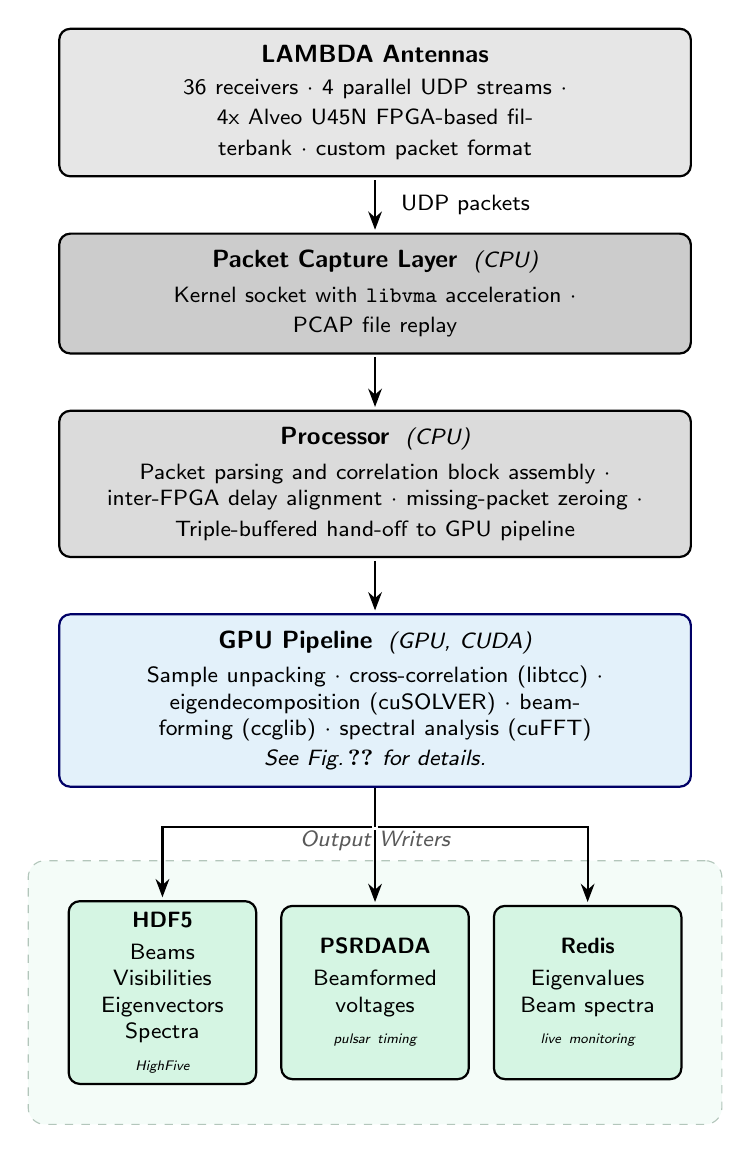
\begin{tikzpicture}[node distance=7mm]

  %% --- Instrument ---
  \node[mbox, fill=cHost!50]
    (inst)
    {\textbf{LAMBDA Antennas}\\[2pt]
     \footnotesize
     36 receivers $\cdot$
     4 parallel UDP streams $\cdot$\\ 
     4x Alveo~U45N FPGA-based filterbank $\cdot$
     custom packet format};

  %% --- Packet Capture ---
  \node[mbox, fill=cHost, below=of inst]
    (cap)
    {\textbf{Packet Capture Layer}
     \;{\footnotesize\itshape(CPU)}\\[3pt]
     \footnotesize
     Kernel socket with \texttt{libvma} acceleration $\cdot$\\
     PCAP file replay};

  %% --- ProcessorState ---
  \node[mbox, fill=cHost!70, below=of cap]
    (proc)
    {\textbf{Processor}
     \;{\footnotesize\itshape(CPU)}\\[3pt]
     \footnotesize
     Packet parsing and correlation block assembly $\cdot$\\
     inter-FPGA delay alignment $\cdot$ missing-packet zeroing $\cdot$\\
     Triple-buffered hand-off to GPU pipeline};

  %% --- GPU Pipeline ---
  \node[mbox, fill=cCuda!35, below=of proc, draw=blue!40!black]
    (gpu)
    {\textbf{GPU Pipeline}
     \;{\footnotesize\itshape(GPU, CUDA)}\\[3pt]
     \footnotesize
     Sample unpacking~$\cdot$ 
     cross-correlation~(libtcc)~$\cdot$ eigendecomposition~(cuSOLVER)~$\cdot$
     beamforming~(ccglib)~$\cdot$ spectral analysis~(cuFFT)\\
     {\itshape See Fig.\,\ref{fig:gpu-pipeline} for details.}};

  %% --- Output writers: three boxes below GPU ---
  \node[wbox] (hdf5) at ([xshift=-27mm, yshift=-26mm]gpu.south)
    {\textbf{HDF5}\\[2pt]
     Beams\\Visibilities\\Eigenvectors\\Spectra\\[2pt]
     {\tiny\itshape HighFive}};

  \node[wbox] (dada) at ([yshift=-26mm]gpu.south)
    {\textbf{PSRDADA}\\[2pt]
     Beamformed voltages\\[2pt]
     {\tiny\itshape pulsar timing}};

  \node[wbox] (redis) at ([xshift=27mm, yshift=-26mm]gpu.south)
    {\textbf{Redis}\\[2pt]
     Eigenvalues\\Beam spectra\\[2pt]
     {\tiny\itshape live monitoring}};

  %% Background box grouping output tier
  \begin{scope}[on background layer]
    \node[draw=cOut!60!gray, dashed, rounded corners=6pt,
          fill=cOut!25, inner sep=5mm,
          fit=(hdf5)(dada)(redis)] (outgrp) {};
  \end{scope}
  \node[above, font=\sffamily\footnotesize\itshape, text=gray!70!black]
    at (outgrp.north) {Output Writers};

  %% Arrows – main flow
  \draw[arr] (inst) -- (cap)
    node[right, midway, xshift=2mm, font=\sffamily\footnotesize]
    {UDP packets};

  \draw[arr] (cap) -- (proc)
    node[right, midway, xshift=2mm, font=\sffamily\footnotesize]
    {};

  \draw[arr] (proc) -- (gpu)
    node[right, midway, xshift=2mm, font=\sffamily\footnotesize]
    {};

  %% Fan-out from GPU to output tier
  \coordinate (fo) at ([yshift=-5mm]gpu.south);
  \draw[thick] (gpu.south) -- (fo);
  \draw[arr]   (fo) -| (hdf5.north);
  \draw[arr]   (fo) --  (dada.north);
  \draw[arr]   (fo) -| (redis.north);

  \end{tikzpicture} \caption{% 
    Overall architecture of the real-time radio-astronomy signal processing
    pipeline.  Incoming UDP packets from the LAMBDA array are captured by the
    packet capture layer, assembled into correlation blocks by the
    \texttt{Processor}, and processed by the \texttt{GPU Pipeline}
    (see Figure\,\ref{fig:gpu-pipeline}).  Depending on the pipeline setup,
    results are written to HDF5 files via HighFive (beams,
    cross-correlation visibilities, eigenvectors, and spectra), to PSRDADA ring
    buffers (beamformed voltages for pulsar timing), and to Redis (beam bandpass for real-time monitoring with Grafana).
    % 
} \label{fig:arch-overview} \end{figure}

\begin{figure}[!htbp]
  \centering
  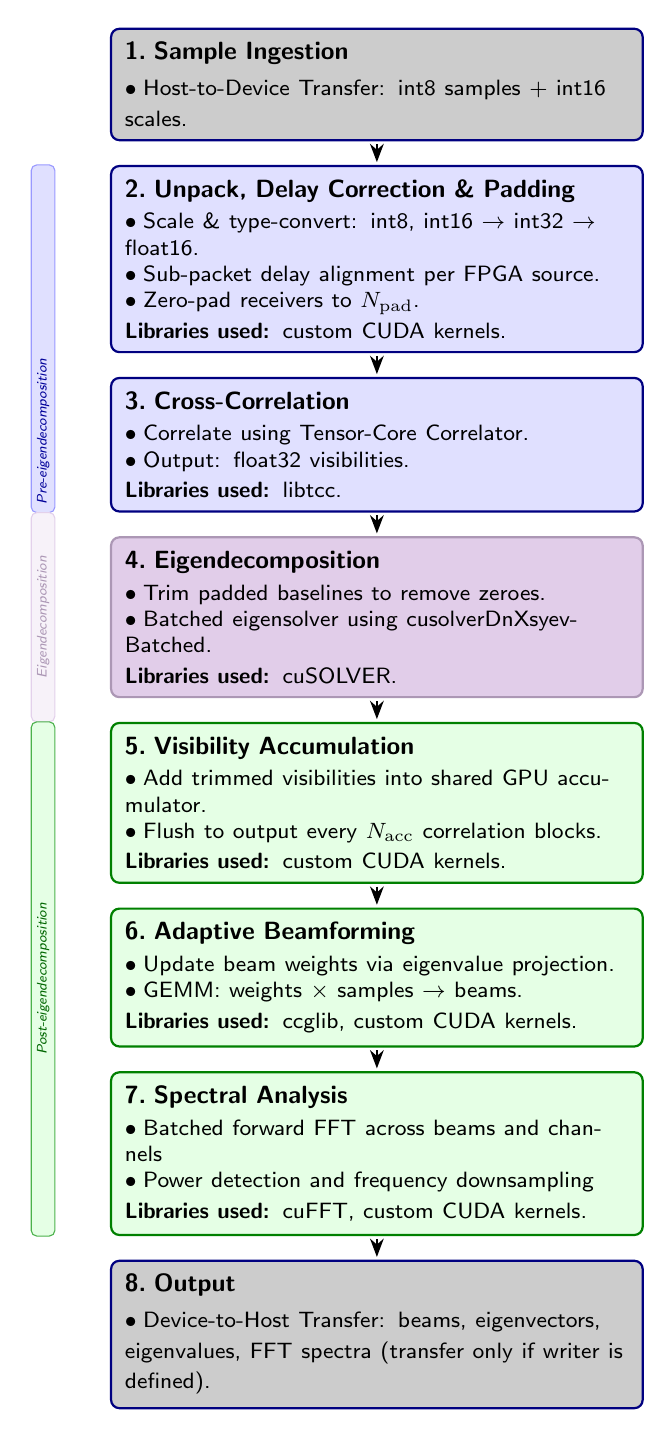
\begin{tikzpicture}[node distance=3mm]

  \node[pbox, fill=cHost, draw=blue!50!black]
    (p1)
    {\textbf{1.\;Sample Ingestion}\\[2pt]
     \footnotesize
     $\bullet$\;Host-to-Device Transfer: int8 samples + int16 scales.
   };

  \node[pbox, fill=blue!12, draw=blue!50!black, below=of p1]
    (p2)
    {\textbf{2.\;Unpack, Delay Correction \& Padding}\\[2pt]
     \footnotesize
     $\bullet$\;Scale \& type-convert: int8, int16 $\to$ int32 $\to$ float16.\\
     $\bullet$\;Sub-packet delay alignment per FPGA source.\\
     $\bullet$\;Zero-pad receivers to $N_\mathrm{pad}$.\\
   \textbf{Libraries used:} custom CUDA kernels.};

  \node[pbox, fill=blue!12, draw=blue!50!black, below=of p2]
    (p3)
    {\textbf{3.\;Cross-Correlation}\\[2pt]
     \footnotesize
     $\bullet$\;Correlate using Tensor-Core Correlator.\\
     $\bullet$\;Output: float32 visibilities.
                \\
          \textbf{Libraries used:} libtcc.};

  \node[pbox, fill=cSolve!75, draw=cSolve!80!black, below=of p3]
    (p4)
    {\textbf{4.\;Eigendecomposition}\\[2pt]
     \footnotesize
     $\bullet$\;Trim padded baselines to remove zeroes.\\
     $\bullet$\;Batched eigensolver using cusolverDnXsyevBatched.\\
     \textbf{Libraries used:} cuSOLVER.};

  \node[pbox, fill=green!10, draw=green!50!black, below=of p4]
    (p5)
    {\textbf{5.\;Visibility Accumulation}\\[2pt]
     \footnotesize
     $\bullet$\;Add trimmed visibilities into shared GPU accumulator.\\
     $\bullet$\;Flush to output every $N_\mathrm{acc}$ correlation blocks.\\
   \textbf{Libraries used:} custom CUDA kernels.};

  \node[pbox, fill=green!10, draw=green!50!black, below=of p5]
    (p6)
    {\textbf{6.\;Adaptive Beamforming}\\[2pt]
     \footnotesize
     $\bullet$\;Update beam weights via eigenvalue projection.\\
     $\bullet$\;GEMM: weights $\times$ samples $\to$
                beams.
                \\
   \textbf{Libraries used:} ccglib, custom CUDA kernels.};


  \node[pbox, fill=green!10, draw=green!50!black, below=of p6]
    (p7)
    {\textbf{7.\;Spectral Analysis}\\[2pt]
     \footnotesize
     $\bullet$\;Batched forward FFT across beams and channels\\
     $\bullet$\;Power detection and frequency downsampling\\
  \textbf{Libraries used:} cuFFT, custom CUDA kernels.};

  \node[pbox, fill=cHost, draw=blue!50!black, below=of p7]
    (p8)
    {\textbf{8.\;Output}\\[2pt]
     \footnotesize
     $\bullet$\;Device-to-Host Transfer: beams, eigenvectors, eigenvalues,
                FFT spectra (transfer only if writer is defined).};

  %% Vertical flow arrows (explicit -- no \foreach)
  \draw[arr] (p1.south) -- (p2.north);
  \draw[arr] (p2.south) -- (p3.north);
  \draw[arr] (p3.south) -- (p4.north);
  \draw[arr] (p4.south) -- (p5.north);
  \draw[arr] (p5.south) -- (p6.north);
  \draw[arr] (p6.south) -- (p7.north);
  \draw[arr] (p7.south) -- (p8.north);

  %% Left-margin section bars (plain \fill + \draw -- no fit, no background scope)
  \fill[blue!12, rounded corners=2pt]
    ([xshift=-10mm]p2.north west) rectangle ([xshift=-7mm]p3.south west);
  \draw[blue!40, rounded corners=2pt]
    ([xshift=-10mm]p2.north west) rectangle ([xshift=-7mm]p3.south west);
  \node[rotate=90, anchor=center, font=\sffamily\tiny\itshape, text=blue!60!black]
    at ($([xshift=-8.5mm]p2.north west)!0.5!([xshift=-8.5mm]p4.south west)$)
    {Pre-eigendecomposition};

  \fill[cSolve!20, rounded corners=2pt]
    ([xshift=-10mm]p5.north west) rectangle ([xshift=-7mm]p3.south west);
  \draw[cSolve!70, rounded corners=2pt]
    ([xshift=-10mm]p5.north west) rectangle ([xshift=-7mm]p3.south west);
  \node[rotate=90, anchor=center, font=\sffamily\tiny\itshape, text=cSolve!80!black]
    at ($([xshift=-8.5mm]p4.north west)!0.5!([xshift=-8.5mm]p4.south west)$)
    {Eigendecomposition};

  \fill[green!10, rounded corners=2pt]
    ([xshift=-10mm]p5.north west) rectangle ([xshift=-7mm]p7.south west);
  \draw[green!40!gray, rounded corners=2pt]
    ([xshift=-10mm]p5.north west) rectangle ([xshift=-7mm]p7.south west);
  \node[rotate=90, anchor=center, font=\sffamily\tiny\itshape, text=green!40!black]
    at ($([xshift=-8.5mm]p5.north west)!0.5!([xshift=-8.5mm]p7.south west)$)
    {Post-eigendecomposition};

  \end{tikzpicture}
  \caption{%
    Processing stages within the GPU pipeline. Each invocation
    processes one assembled buffer comprising $N_\mathrm{pkt}$ packets
    across $N_\mathrm{ch}$ frequency channels and $N_\mathrm{fpga}$ FPGA
    sources.  Left-margin bars and box border colours indicate the three
    pipeline sections: stages~2--3 (\textcolor{blue!60!black}{blue} border,
    pre-eigendecomposition) and stages~5--7
    (\textcolor{green!50!black}{green} border, post-eigendecomposition) are
    each captured into a CUDA graph to minimise kernel launch overhead;
    stage~4 (\textcolor{cSolve!80!black}{violet} border) executes separately
    because \texttt{cusolverDnXsyevBatched} performs host-side work
    that cannot be captured. Each stage can be made up of multiple GPU kernels. 
    cuTENSOR tensor permutations are used throughout
    the pipeline to manipulate memory to meet input requirements of different 
    libraries.
    Abbreviations: $N_{pad}$, number of received padded up to nearest multiple of 32; 
    $N_{acc}$, number of correlation blocks to accumulate before outputting.
  }
  \label{fig:gpu-pipeline}
  \end{figure}

The relatively low number of elements and dense packing of elements means that
the processing requirements are relatively modest. There are opportunities for
a flexible implementation of spatial filtering to figure out what works and
what does not.

\cite{astron_lofar_2026} shows the LOFAR minimum integration time is
approximately 0.5 seconds.

LOFAR uses an entirely GPU-based system - no FPGAs
(\cite{broekema_cobalt_2018}).

SKAO integration time is about 283 ms (\cite{skao_low_2026}).

The integration time of 17.7 ms is already the finest time resolution
available. The system is also extremely flexible, with new modes and pipelines
easy to extend through software alone.

\subsection{Benchmarks}
We present here benchmarks of the CPU and GPU portions of the pipeline. 
Each part was benchmarked in three environments: 
\begin{enumerate}
\item the LAMBDA production environment at Narrabri, consisting of a server with 2$\times$ Intel Xeon 4210 CPUs and 1$\times$ NVIDIA RTX 4000 Ada GPU. 
\item Ngarrgu Tindebeek supercomputer at Swinburne University, a HPC cluster with A100 GPUs.
\item a development machine owned by the author, with a Ryzen 7 7700 CPU and a NVIDIA 4060 GPU.
\end{enumerate}

While all of the benchmarks were run in each environment, we present the production environment against the best secondary benchmark. 
This is because not all environments are optimized for each type of test. For example, the CPU processing struggled on the Ngarrgu Tindebeek node, while 
the 4060 performance was clearly inferior to the A100.

We present benchmarks in input GB/s for a range of channels between 8 and 32, or 6.25 - 25 MHz of usable bandwidth. 
We use a fixed correlation block size of 256 packets per channel per FPGA, which corresponds to 17.7 ms.
Memory and compute scaling for the pipeline is linear in the number of channels.
We fix the number of receivers at the current size of the array to be 36 antennas + 4 null streams to make 40 receivers.

We present benchmarks for two GPU pipelines: the full pipeline including beamforming, correlation, and RFI mitigation; and a simplified version with only correlation and beamforming. 
The GPU pipelines were exercised by filling input buffers on the CPU, and repeatedly calling the GPU pipeline over a 30 second period. The actual runtime was recorded
and the total number of pipeline runs was divided by the runtime to give the average runs per second. Warm-up calls of the pipeline which included the just-in-time (JIT) compilation of the \texttt{libtcc} and \texttt{ccglib} kernels were carried out before the 30 second period, to avoid these skewing the results.

The CPU processor consists of parsing captured packets and sorting them into correlation blocks for processing on the GPU.
It was benchmarked by having a set of producer threads, mimicing the packet-capture threads in the production deployment, generate synthetic packets and input them 
to the processor's input buffer. 
The benchmark script captures the number of packets processed by the processor over a 30 second period and uses this to calculate the GB/s throughput.
The results of both the CPU and GPU throughputs are shown in Figure~\ref{fig:gpu-throughput}.

Given the data rates in Table~\ref{data-flows-lambda}, one A100 GPU would be sufficient to carry out RFI mitigation in addition to correlation and beamforming for the current array and the entire 65 MHz of processed bandwidth. When expanded to the full 256 antennas, four A100s would be sufficient for the 65 MHz processed bandwidth.


We also present profiling of the largest six CUDA kernels by average runtime through NSight-Compute and Nsight-Systems analysis. This was carried out on the 4 FPGA, 32 channel 
configuration.
These kernels are:
\begin{itemize}
	\item \texttt{correlate}: from \texttt{libtcc} which carries out correlation.
	\item \texttt{wmma\_complex\_gemm\_opt} from \texttt{ccglib}, this is the beamforming step.
	\item \texttt{transpose} from \texttt{ccglib} which rearranges the input tensor for optimal use of tensor cores.
	\item \texttt{tensor\_permute}
	\item \texttt{scale\_and\_convert\_to\_half\_kernel}: a custom kernel which converts the input samples and scales to \texttt{int32}, multiplies them, and converts to half-precision floating point for further processing.
	\item \texttt{apply\_delays}: a custom kernel that compensates for the fine delay calibration between different FPGAs.
\end{itemize}



\begin{figure}
	\centering
	\includegraphics[width=\columnwidth]{images/comparison_gpu_channel_sweep.png}
	 \vspace{2mm}
	 \includegraphics[width=\columnwidth]{images/comparison_processor_channel_sweep.png}
	\caption{
		(a) Throughput of the GPU pipelines in isolation. CorrBeam-only is a pipeline that only does correlation and beamforming steps. RFIMit is the pipeline that includes eigendecomposition and weight updates in addition to correlation and beamforming. Results are shown for both the production server's RTX 4000 Ada Generation, and an A100 on the Ngarrgu Tindebeek supercomputer at Swinburne University. We also show the real-time required GB/s for the current array configuration with varying number of channels.\\
		(b) Throughput of the CPU packet processor in isolation. The Xeon 4210 is from the LAMBDA production environment at Narrabri, while the AMD Ryzen 7 7700 is from the development machine. This suggests that the system will benefit from more recent hardware with a higher clock speed.
	}
	\label{fig:gpu-throughput}
\end{figure}

\begin{figure*}
	\centering
	\includegraphics[width=\textwidth]{images/profile_overview.png}
	\caption{Profiling results of the top six kernels by execution runtime from an A100 on Ngarrgu Tindebeek. From left-to-right, top-to-bottom, we show: (a) total execution time of the kernel in microseconds, (b) tensor-core utilisation, (c) theoretical and achieved warp occupancy, and (d) compute and memory throughput. We show the results for a fixed configuration of 4 FPGAs (40 receivers) and 32 channels for an input data rate of 5 GB / s.}
	\label{fig:gpu-profiling}
\end{figure*}



\section{A simplified test for interference subspace detection}

A number of tests are laid out in \cite{van_trees_optimum_2002} for the detection of
the interference subspace, including tests based upon sequential hypothesis testing, 
and penalty-based tests like the Akaike Information Criterion (AIC).

These tests work similarly - interfering signals are detected through comparing
the largest eigenvalues to the remaining, smaller, eigenvalues. Under the model, 
a certain number of eigenvalues will just be noise with common power $\phi^{2}$.
We use $\phi$ to avoid confusion with use of $\sigma$ as a standard deviation 
in the remainder of this section.

These tests were created with a variety of fields in mind; however, for the
purposes of radio astronomy, we can create a simplified threshold test.

Under the following assumptions:
\begin{enumerate}
    \item the number of receivers $N$ is much greater than the number of interfering signals $k$:  $N >> k$.
    \item the time resolution of visibilities is such that subspace smearing is not an issue.
\end{enumerate}

Subspace smearing causes a small number of interferers to contaminate a much greater 
number of eigenvalues.

If this is the case, then we can assume that the median eigenvalue will be a
good estimate of the noise power. We then take a measurement of the standard deviation of the 
noise eigenvalues and apply a configurable thresholding approach to detect the number of signal eigenmodes.

For the spread measurement, we take all eigenvalues between the 20th and 80th percentile and take the 
range. We then scale this up assuming a Gaussian distribution for the noise eigenvalues.

\begin{equation}
  \Sigma_{noise} = \frac{p_{80} - p_{20}}{2 \times 0.8416}
\end{equation}

where $0.8416$ is the $Z$-score corresponding to a tail area of $0.2$.

We choose to take the 20th percentile cutoff as flagged antennas show as zero eigenvalues in the implementation.

A threshold is then defined as 
\begin{equation}
  T = p_{50} + \Delta \times \Sigma_{noise}
\end{equation}
with all eigenvalues exceeding this threshold being taken as interfering eigenmodes.

\subsection{Sky Model}
A common worry with eigenmode methods is that legitimate signals of interest
will be removed accidentally. This is certainly possible in schemes where
a certain number of eigenvalues are nulled every time period.

During the day, the sun is flagged as part of this interference subspace. However we know the 
direction of the sun relative to the array, so we can compute its spatial signature.
We can therefore remove the sun's contribution from the interference subspace to avoid 
nulling a celestial source of interest.
Equivalently - we can add it back to the noise subspace to remove the null in the direction of the sun.

\begin{equation}
 P_{n} = b b^{*} + \sum_{j \in \text{noise}} v_j v_{j}^{*}
\end{equation}
where $P_{n}$ is the orthogonal projector into the noise + celestial source subspace, $v_{j}$ are 
eigenvectors of $R$, and $b$ is the known steering vector of the sun.


It can sometimes be the case that we actually do want to null the sun, in which case 
removing the sun from the interference subspace is not required.

For a more sensitive telescope, if a sky model is known then bright sources can be explicitly tested 
if they fall into the interference subspace, and if so, their direction added back into the noise projection
matrix.



\section{Results of Spatial Filtering experiments}
We used LAMBDA to test the effectiveness of spatial filtering in three experiments 
of increasing complexity.
\begin{enumerate}
    \item Nulling of an injected synthetic interferer in an otherwise clean sky channel.
    \item Nulling of an FM radio station, a stationary interferer with respect to the array.
    \item Nulling of an Low-Earth Orbit (LEO) Orbcomm satellite.
  \end{enumerate}

In each case, the array was first calibrated using the following procedure:
\begin{enumerate}
  \item \textbf{Inter-FPGA delay calibration}: A sample of packets arriving from each
    FPGA was captured and the ``optimal lag" between each FPGA and a reference FPGA 
    computed in order to align samples from all FPGAs to the nearest time sample.
    This assumes that the brighest source is the same amongst all antennas, a reasonable assumption due to 
    the compactness of the array. 
    Once calibrated, this time sample delay is constant until reboot of any FPGA.
  \item \textbf{Antenna gain calibration}: The sun was used as a calibration source
    using the quiet-sun model. Model visibilities were created over a 90 second period to
    estimate the antenna gains. These gains also include the sub-sample delay correction for 
    inter-FPGA baselines.
  \end{enumerate}

For results showing bandpasses, all mitigation work was completed in real-time using the pipeline.

For imaging results, data was collected using the pipeline and visibilities output to HDF5. 
The mitigation and imaging was then completed offline.
All images shown are dirty images taken by discrete Fourier transform of the visibilities using 
the antenna positions.

The detection test of Section~(insert num) has only been used in the imaging steps
for the Orbcomm satellite and is not currently implemented in the GPU pipeline.




\subsection{Removal of synthetic RFI}

We firstly validate the RFI mitigation by removing a synthetic interferer from 
an otherwise clean bandpass.

The LAMBDA ADCs have a feature to add a simulated pulse train to the processed data. 
This pulse train shows up as a picket-fence in frequency with an approximate
spacing of 300 kHz (check exact with Joseph).

This pulse train arrives with a per-antenna delay which means that it folds
neatly into one dominant eigenmode. This is because within one coarse channel a
fixed delay is a constant phase per antenna. The pulse is also more powerful
than the background sky noise, so removal of the dominant eigenmode should
recover the sky noise.

This experiment validates that the pipeline works to correctly mitigate an
injected RFI source without changing the rest of the bandpass materially. Due
to the hard-coded nature of nulling the dominant eigenmode it does not test the
detection test of Section~whatever it is.

For this experiment, we chose an otherwise RFI-free channel and injected the
synthetic pulse train. We then set the beamformer to use unity weights and
mitigate the dominant eigenmode. Unity weights were chosen for simplicity
because there is no real sky source to point at. Even though there is no
motion, weights were re-calculated every 256 packets containing 64 time steps
each at a time resolution of 1.08 $\mu$s, for an update time of 17.69 ms.

We show the bandpass of one coarse channel in
Figure~\ref{fig:synthetic-bandpass}. The three spikes from the pulse train are
clearly visible in the unmitigated bandpass. We also see the mitigated bandpass
tracks the unmitigated bandpass in areas outside of the pulse train, but
cleanly interpolates in the pulse train spikes. In clean sections of the bandpass,
the difference between the mitigated and unmitigated signals is two orders of magnitude
below the level of the noise.


It is also worth noting that due to the fact there is no motion in the pulse train,
smearing is not a concern here. Therefore the integration time or weight update time
is irrelevant in this experiment.


\begin{figure}
    \centering
        \includegraphics[width=\columnwidth]{images/bandpass_fft_ch2_pol1_4096fft_4096bins.png}
        \vspace{2mm}
        \includegraphics[width=\columnwidth]{images/bandpass_difference_fft_beam1_minus_beam0_ch2_pol1_4096fft_4096bins.png}
    \caption{Mitigated (orange) and unmitigated (blue) bandpass for a single coarse channel split into 
      4096 fine channels. This has 3 eigenmodes removed.
      The power difference between the mitigated and unmitigated beams in the clean areas is 3.1 dB.
      This reduces the interfering signals by 30 dB for the first, and 28 dB for the second. It also mitigates 
      two RFI spikes from the sky noise.
    }
    \label{fig:synthetic-bandpass}
\end{figure}



\subsection{Beamforming and imaging while mitigating FM radio station}

The next experiment is to test spatial filtering methods for imaging and 
beamforming is to null a static RFI source in real-time. 
As LAMBDA is a ground-based driftscan aperture array, FM radio stations are a 
fixed source of RFI with respect to the array. 

These FM radio stations are also enormously powerful.

At the observatory site in Narrabri, there is a FM transmitter approximately 60 km
as the crow flies east in the Mount Kaputar National Park.

However in the data we also see FM radio stations on frequencies that are not
broadcast from the Mt. Kaputar station. These may be carried from transmitters 
further afield by atmospheric ducting.

The mitigation resulted in a reduction in the interferer power of approximately 
20 dB.

Currently we see a reduction in power over the entire bandpass - hypothesise that this is due to the FFT 
to create the fine channels - the FM radio is so powerful it leaks into the 
other bins - need to check this.


\begin{figure}
    \centering
        \includegraphics[width=\columnwidth]{images/fm-radio-over-time.png}
        \vspace{2mm}
        \includegraphics[width=\columnwidth]{images/fm-radio-time-averaged.png}
    \caption{
    (a) Bandpass over time for a single coarse channel split into 64 fine channels.
      (b) Mitigated (orange) and unmitigated (blue) bandpass for a single coarse channel split into 
    55 fine channels.}
    \label{fig:fm-bandpass}
\end{figure}


\begin{figure}
    \centering

        \includegraphics[width=\columnwidth]{images/20260512-dirty-image-no-RFI.png}
        \vspace{2mm}
        \includegraphics[width=\columnwidth]{images/20260512-dirty-rfi-image.png}
        \vspace{2mm}
        \includegraphics[width=\columnwidth]{images/20260512-dirty-image-shrunk.png}
    \caption{(a) Actual dirty image of sky from adjacent clean channel.\\
    (b) Dirty image of the sky with unmitigated FM radio interference.\\
  (c) Recovered image of the sky using eigenvalue shrinking.}
    \label{fig:fm-radio-imaging}
\end{figure}


\begin{figure}
    \centering
        \includegraphics[width=\columnwidth]{images/sun-peeling.png}
    \caption{Peeling the sun shows the galactic plane underneath.}
    \label{fig:sun-peeling}
\end{figure}



\subsection{Imaging while mitigating Orbcomm satellite}
Orbcomm satellites transmit at approximately 137.5 MHz.
They are in low-Earth orbit and have an orbital period of approximately 100 minutes.

A time was chosen where no Orbcomm satellite was visible from the LAMBDA site.
Three satellites were visible over the next 15 minutes, before they all set.
This allowed RFI-free opportunity for calibration of the array.

Visibilities were dumped to disk at a 17.7 ms time resolution. 

Dirty images were formed for the purposes of seeing the satellite motion, and a 
movie was created that shows one of the satellites moving through the sky. 
Its motion is concordant with its expected trajectory from gpredict.

To mitigate the satellite, at each time step we used the test of section (insert section) to detect the 
interference subspace and project the data into the noise + sun subspace. 
We then integrated these short term visibilities to various time resolutions and 
imaged them again to recover the expected sky image.


\begin{figure*}
    \centering
    \includegraphics[width=\textwidth]{images/comparison-rfi-vs-corrected.png}
    \caption{From left-to-right, top-to-bottom:\\
    (a) No RFI-mitigation applied.\\
  (b) An adjacent RFI-clean channel contemporaneous observation. \\
(c) RFI-mitigation applied without the Leshem correction applied.\\
(d) RFI-mitigation applied with the Leshem correction applied.}
    \label{fig:rfi-comparison}
\end{figure*}



\section{Conclusions and Future Work}

\section*{Data Availability}

Code can be found at \url{https://github.com/jdgsmallwood/lambda-commissioning} and 
\url{https://github.com/jdgsmallwood/cuda-spatial-filtering}.

Move these to Zenodo




\bibliographystyle{paslike}

\bibliography{PhD}
\end{document}
